\documentclass[11pt,a4paper]{article}
\usepackage[utf8]{inputenc}
\usepackage[T1]{fontenc}
\usepackage{amsmath}
\usepackage{newpxtext,newpxmath}
\renewcommand{\ttdefault}{lmtt}
\usepackage[a4paper,margin=1in]{geometry}
\usepackage{booktabs,longtable,array,calc}
\usepackage{graphicx}
\usepackage{flafter}
\usepackage{fancyvrb}
\usepackage{xcolor}
\definecolor{btred}{HTML}{E63946}
\colorlet{linkred}{btred!82!black}
\usepackage[colorlinks=true,linkcolor={linkred},citecolor={linkred},urlcolor={linkred}]{hyperref}
\usepackage{caption}
\DeclareCaptionLabelSeparator{bar}{\ \textbar\ }
\captionsetup{font=small,labelsep=bar,justification=justified,singlelinecheck=false}
\usepackage{titlesec}
\titleformat{\section}{\large\bfseries}{\thesection.}{0.5em}{}
\titleformat{\subsection}{\normalsize\bfseries}{\thesubsection}{0.6em}{}
\titlespacing*{\section}{0pt}{2.2ex plus .6ex minus .3ex}{1ex}
\titlespacing*{\subsection}{0pt}{1.8ex plus .5ex minus .2ex}{0.8ex}
\usepackage{etoolbox}
\AtBeginEnvironment{longtable}{\small\setlength{\tabcolsep}{4pt}\hyphenpenalty=10000\exhyphenpenalty=10000}
\setlength{\emergencystretch}{3em}
\linespread{1.05}
\usepackage{xurl}
\usepackage[skip=0.55\baselineskip plus 2pt]{parskip}
\usepackage{tcolorbox}
\newtcolorbox{codebox}{colback=black!3,colframe=black!15,boxrule=0.4pt,arc=2pt,left=7pt,right=7pt,top=2pt,bottom=2pt,
  before skip=6pt,after skip=8pt}
\providecommand{\tightlist}{\setlength{\itemsep}{0pt}\setlength{\parskip}{0pt}}
\setlength{\LTcapwidth}{\textwidth}
\renewcommand{\arraystretch}{1.1}
\begin{document}
\thispagestyle{plain}
\noindent
\includegraphics[width=\textwidth]{bt_header.pdf}\par\nointerlineskip
\vspace{4pt}\hrule height 0.4pt\relax
\vspace{18pt}
\begin{center}
{\LARGE\bfseries Dirty L2, Drained Queues:\\[3pt] Measurement Pitfalls in GPU Kernel Microbenchmarks\par}
\vspace{12pt}
\begin{tabular}{@{}c@{\hspace{2.2em}}c@{}}
Rungrod Thongjampa & Chanchada Wathanathonnan \\[1pt]
{\small\texttt{rungrod.th@blacktile.dev}} & {\small\texttt{chanchada.wa@blacktile.dev}}
\end{tabular}\\[6pt]
Blacktile Research \quad\textperiodcentered\quad {\small November 2026}
\vspace{12pt}

{\Large\bfseries Abstract}
\end{center}
\vspace{-4pt}
GPU kernel microbenchmarks evict cached inputs before each timed call. In 14 of the 15 tools and benchmark paths we
audited, including \texttt{triton.testing.do\_bench}, the eviction writes a large buffer. The writes leave dirty L2 lines
that the timed kernel must write back, so the flush changes the measurement. With pre-registered experiments on
nine NVIDIA GPUs, a batch-1 fp16 decode GEMV measured 6.6-25.3 \% slower with the shipped write flush than with a
read flush, and the bias changed which quantized GEMV appeared faster on some GPUs. Hardware counters on a laptop
GPU confirm the mechanism. Two related pitfalls follow: a flush shorter than the host\textquotesingle s dispatch time lets the
command queue drain, so a CUDA-event interval includes host time; and a read flush leaves the measured kernel\textquotesingle s own
write-back untimed. Against a four-layer, GEMV-only decode proxy captured in a CUDA graph, summed shipped do\_bench
times over-predicted the step by 26-32 \% (fp16) on GPUs with large L2 and mis-ranked int4 kernels on an RTX 4060.
Timing kernels from CUPTI activity timestamps over a CUDA graph that rotates through weight copies matched the same
kernels inside the proxy within 0.79 \% (12 kernels, ratio of medians over three runs) on one clock-locked laptop
GPU. This agreement was not reproduced on rented RTX 4060 and A100 hosts, which refused clock locking: clock
changes, a kernel-context effect and tracing overhead limited it. We release a harness with explicit quality gates
and list the hazards we measured.

\begin{center}
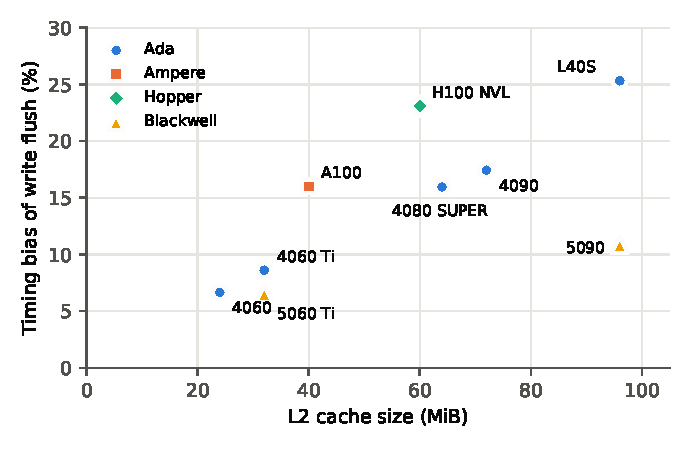
\includegraphics[width=0.56\textwidth]{fig_bias_vs_l2.pdf}
\end{center}
\vspace{-10pt}
\captionof{figure}{Timing bias of the shipped write flush relative to a read flush, for a batch-1 fp16 decode GEMV
(112\,MiB of weights), on nine GPUs. Within Ada the bias rises with L2 size; A100 and H100 sit above the Ada
trend, Blackwell below. Values are in the table of Section~5; the four GPUs with $\ge$64\,MiB of L2 are scored
under the amended validity check (Section~13).}\label{fig:bias}
\vspace{2pt}\noindent\rule{\textwidth}{0.4pt}
\par\medskip
\section{Summary for practitioners}\label{summary-for-practitioners}

If you time memory-bound GPU kernels (decode GEMV/GEMM, attention decode, norms, activations, quantized
matmuls) or compare kernels that move different numbers of bytes:

\begin{enumerate}
\def\labelenumi{\arabic{enumi}.}
\tightlist
\item
  \textbf{Flush the L2 by reading, not writing.} A write leaves dirty lines that your kernel then writes back (\hyperref[how-big-is-the-bias-nine-gpus]{\S{}5}).
\item
  \textbf{Read a buffer well above the L2 size.} Our conservative default is max(256~MiB, 4 \ensuremath{\times} L2); an L2-sized read
  left part of the previous call\textquotesingle s output dirty, and 2 \ensuremath{\times} L2 was not enough for short kernels with large outputs
  (\hyperref[what-removes-the-residue-and-what-does-not]{\S{}6}). Check it for your output sizes.
\item
  \textbf{Keep the GPU busy before the start event.} If the flush finishes before the host has enqueued your
  kernel, you time the host (\hyperref[pitfall-2-queue-drain]{\S{}7}). nvbench does this with a blocking kernel; in Python, one line after the flush
  removed it in our measurements: \texttt{torch.cuda.\_\allowbreak{}sleep(cycles)}.
\item
  \textbf{In a per-call cold loop, do not wait (synchronize, sleep) between flush and timing.} Dirty lines stayed dirty
  while the GPU was idle, and the queue drains (\hyperref[what-removes-the-residue-and-what-does-not]{\S{}6}, \hyperref[pitfall-2-queue-drain]{\S{}7}).
\item
  \textbf{Decide who pays for writes.} A cold, read-flushed time leaves part of the kernel\textquotesingle s own write-back untimed
  (about L2/2 on our laptop GPU, more on an L40S). For kernels that write, report a steady-state time as well (\hyperref[pitfall-3-who-pays-for-a-kernels-own-writes]{\S{}8}).
\item
  \textbf{For a kernel\textquotesingle s eventual DRAM write traffic from Nsight Compute, profile one range that ends with a full L2
  flush after the kernel, with a synchronization}; per-kernel counters can miss the write-back (\hyperref[measurement-pitfall-per-kernel-dram-write-counters-lose-bytes]{\S{}11}).
\item
  \textbf{When a per-kernel number should match the kernel inside a model, time it from CUPTI timestamps over a CUDA
  graph that rotates inputs, after a warm-up, and check the conditions:} tracing must not change the graph\textquotesingle s time
  (\ensuremath{\le} 0.5~\%), the clock must be steady, and the context must resemble the model\textquotesingle s. Under these conditions, on one
  clock-locked laptop GPU, this matched 12 kernels of a GEMV-only decode proxy within 0.79~\%; where they failed, it
  was off by up to 14~\% (\hyperref[kernel-by-kernel-does-a-single-kernel-benchmark-match-the-same-kernel-inside-the-decode-proxy]{\S{}9.1}). If the conditions cannot be met, time the model\textquotesingle s own graph. CUPTI timing is not
  new (FlashInfer has it, \hyperref[related-work-and-credit]{\S{}14}).
\item
  \textbf{Make the clock steady, or report how much it moved.} Lock the SM clock where you may (\texttt{nvidia-smi\ -lgc}, root
  only; rented containers refused). For small changes, a relative clock change \(\Delta f/f\) changes a kernel\textquotesingle s time
  by about \(-s\,\Delta f/f\), where \(s\) is the share of its time that scales with the SM clock: near 0 for the
  memory-bound fp16 GEMVs and roughly 0.6-0.9 for int4 and NF4 GEMVs on our laptop GPU (\hyperref[kernel-by-kernel-does-a-single-kernel-benchmark-match-the-same-kernel-inside-the-decode-proxy]{\S{}9.1}, post hoc and rough).
\item
  \textbf{Tune on the machine you deploy on.} Two hosts with the same H100 NVL ran the same decode step 9-27~\% apart (\hyperref[end-to-end-check-which-number-predicts-a-decode-step]{\S{}9}).
\end{enumerate}

\texttt{cleanbench} (\hyperref[cleanbench]{\S{}10}) does 1-3, 5 and 7, reports whether the conditions of item 7 held, and warns when a kernel is too
short for the event timer.

\section{Background}

\begin{figure}[tbp]
\centering
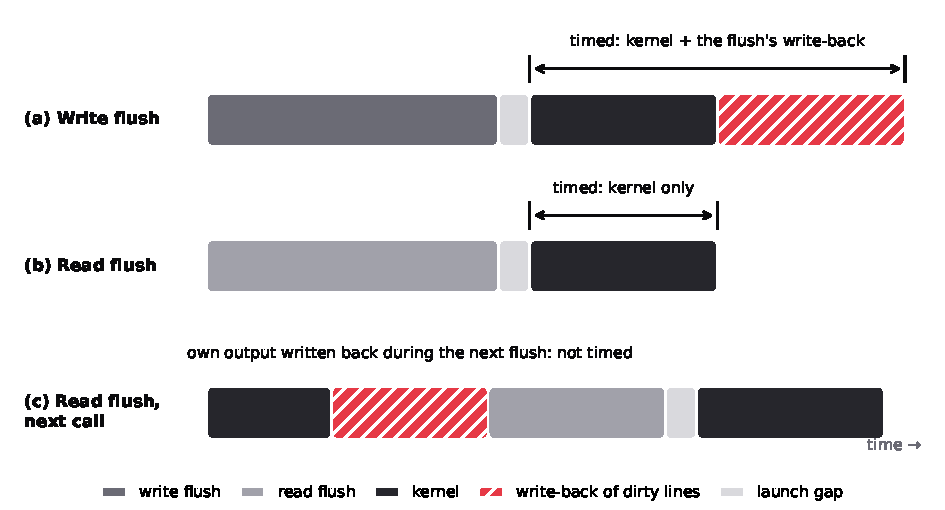
\includegraphics[width=0.92\textwidth]{fig_dirty_l2.pdf}
\caption{Who pays for dirty L2 lines (schematic; in practice the write-back overlaps the kernel). (a) A write flush
leaves dirty lines that the timed kernel must write back. (b) A read flush leaves the L2 clean. (c) Under a read
flush, a kernel's own output stays dirty and is written back during the next flush, outside any timed window.}
\label{fig:dirty}
\end{figure}
\label{background}

\begin{itemize}
\tightlist
\item
  \textbf{Write-back L2.}

  \begin{itemize}
  \tightlist
  \item
    On NVIDIA GPUs stores allocate in L2 and reach DRAM later. A line written but not yet in DRAM is \emph{dirty}.
  \item
    On four dies we measured with DRAM counters, the L2 starts writing dirty lines back, without evicting them,
    once they exceed between 0.44 and 0.63 of its capacity (\hyperref[measurement-pitfall-per-kernel-dram-write-counters-lose-bytes]{\S{}11} has the table). NVIDIA\textquotesingle s US patent 9,639,466
    describes a programmable dirty threshold (from its description; we have not analysed the claims).
  \item
    A dirty line that is evicted must be written back first, by whichever access needs its slot.
  \end{itemize}
\item
  \textbf{Why tools flush.} A kernel timed repeatedly would find its inputs already in L2. Tools therefore stream a
  large buffer through the L2 before every timed call.
\item
  \textbf{The timing loop.} \texttt{do\_\allowbreak{}bench} and most Python tools run, per sample:
  \texttt{flush();\ start.record();\ fn();\ end.record()}, with no synchronization. A CUDA event is timestamped when the
  GPU reaches it in the stream, not when the host records it.
\item
  \textbf{Three things can go wrong}, and they are independent:

  \begin{enumerate}
  \def\labelenumi{\arabic{enumi}.}
  \tightlist
  \item
    the flush leaves dirty lines, which the timed kernel writes back (\hyperref[how-big-is-the-bias-nine-gpus]{\S{}5}, \hyperref[what-removes-the-residue-and-what-does-not]{\S{}6});
  \item
    the flush ends before the host has enqueued \texttt{fn}, so the GPU reaches the start event early (\hyperref[pitfall-2-queue-drain]{\S{}7});
  \item
    the timed kernel\textquotesingle s own output stays dirty and is written back after the end event (\hyperref[pitfall-3-who-pays-for-a-kernels-own-writes]{\S{}8}).
  \end{enumerate}
\end{itemize}

\section{Who is affected: a survey of 15 benchmarking tools}\label{who-is-affected-a-survey-of-15-benchmarking-tools}

We selected tools that LLM-kernel developers commonly use to time or autotune kernels: compiler autotuners, the
benchmark helpers of kernel libraries, serving engines\textquotesingle{} benchmark scripts and kernel leaderboards. The unit is a tool
or benchmark path, not a random sample, so "14 of 15" describes this selection, not a prevalence. We read the timing
code at each project\textquotesingle s \texttt{main} branch on 2026-11-06. Seven entries (Triton,
Inductor, nvbench, CUTLASS, FlashInfer, DeepGEMM, KernelBench) were re-checked in source; the other eight were read
once. Permalinks for all entries are in the artifact. Our measurements used Triton 3.3.1, whose \texttt{do\_\allowbreak{}bench} flush is
the same as on \texttt{main}.

{\small
\begin{longtable}[]{@{}>{\raggedright\arraybackslash}p{(\linewidth - 8\tabcolsep) * \real{0.413}}>{\raggedright\arraybackslash}p{(\linewidth - 8\tabcolsep) * \real{0.101}}>{\raggedright\arraybackslash}p{(\linewidth - 8\tabcolsep) * \real{0.304}}>{\raggedright\arraybackslash}p{(\linewidth - 8\tabcolsep) * \real{0.182}}@{}}
\toprule\noalign{}
Tool & Flush by default & Operation & Buffer \\
\midrule\noalign{}
\endhead
\bottomrule\noalign{}
\endlastfoot
Triton \texttt{triton.testing.do\_\allowbreak{}bench} (main, v3.9.0) & yes & write (\texttt{zero\_\allowbreak{}}) & 256~MiB \\
PyTorch Inductor \texttt{InductorBenchmarker} (default autotuning benchmarker) & yes & write (\texttt{zero\_\allowbreak{}}) & = L2 size \\
NVIDIA nvbench (cold measurements) & yes & write (\texttt{cudaMemsetAsync}) & = L2 size \\
CUTLASS CuTe DSL \texttt{tune} (\texttt{use\_\allowbreak{}cold\_\allowbreak{}l2}) & yes & write (\texttt{cuMemsetD32Async}) & = L2 size \\
FlashInfer \texttt{bench\_\allowbreak{}gpu\_\allowbreak{}time} (\texttt{cold\_\allowbreak{}l2\_\allowbreak{}cache=True}) & yes & write (\texttt{zero\_\allowbreak{}}) & 2 \ensuremath{\times} L2 \\
DeepGEMM \texttt{bench\_\allowbreak{}kineto} & yes & write (\texttt{zero\_\allowbreak{}}) & 256~MB \\
tritonbench, Liger-Kernel benchmarks & yes & via Triton \texttt{do\_\allowbreak{}bench} & 256~MiB \\
Helion autotuner (modes \texttt{call} / \texttt{replay}) & yes & write & 256~MiB \\
vLLM \texttt{benchmarks/} (no shared helper) & per script & write in 19 files & 256~MiB or 2 \ensuremath{\times} L2 \\
SGLang \texttt{marker.do\_\allowbreak{}bench} / \texttt{bench\_\allowbreak{}kineto} & yes & write & 5 \ensuremath{\times} L2 / 8~GB \\
KernelBench (evaluates LLM-written kernels) & yes & write (\texttt{fill\_\allowbreak{}}) & 256~MiB \\
GPU MODE reference-kernels (leaderboard evaluation) & yes & write (\texttt{randn}) & 4~GiB / 256~MiB \\
QuACK benchmark scripts & yes & write & 256~MiB \\
TileLang \texttt{do\_\allowbreak{}bench} & yes & \textbf{read} (fixed 2026-11-04, \#3534~\cite{tilelang3534}) & 256~MiB \\
QuACK autotuner, FlashInfer CUDA-graph path, Triton \texttt{do\_\allowbreak{}bench\_\allowbreak{}cudagraph} & --- & no flush / input rotation & --- \\
\end{longtable}
}

Fourteen of the 15 write the flush buffer in at least one common timing path. Three (Inductor, nvbench,
CUTLASS) use a buffer of exactly L2 size, which matters for \hyperref[what-removes-the-residue-and-what-does-not]{\S{}6} and \hyperref[pitfall-2-queue-drain]{\S{}7}.

\section{Method}\label{method}

\begin{itemize}
\tightlist
\item
  \textbf{Pre-registration.} For every experiment, rules, thresholds and predictions were written and locked (sha256
  of code and predictions, plus a git commit) before any GPU was rented or any value was read. Pipeline checks
  before a lock printed only counts, never measurements. Some hypotheses were motivated by earlier results: the
  queue-drain test (\hyperref[pitfall-2-queue-drain]{\S{}7}) and the harness validation (\hyperref[cleanbench]{\S{}10}) were registered after laptop results suggested them, and
  were then scored on new data. In the nine-GPU study, pilot values were seen before its two amendments, and one
  amendment was written after seeing a single GPU (\hyperref[negative-results-deviations-and-limitations]{\S{}13}). The main wrong predictions are listed in \hyperref[negative-results-deviations-and-limitations]{\S{}13}.
\item
  \textbf{Hardware.}

  \begin{itemize}
  \tightlist
  \item
    Timing: rented docker containers on vast.ai (nine GPUs; then an A100-SXM4-40GB, an RTX 5090, an L40S, an RTX 4060
    and an H100 NVL on new hosts for \hyperref[pitfall-2-queue-drain]{\S{}7}-\hyperref[cleanbench]{\S{}10}), with unlocked clocks.
  \item
    Per-kernel check (\hyperref[kernel-by-kernel-does-a-single-kernel-benchmark-match-the-same-kernel-inside-the-decode-proxy]{\S{}9.1}): the laptop GPU, with and without an SM clock lock at 1,000~MHz (\texttt{nvidia-smi\ -lgc}), and
    rented RTX 4060 and A100-SXM4 hosts, which refused clock locking.
  \item
    Counters: an RTX 3060 Laptop GPU (GA106, L2 3~MiB) with Nsight Compute 2024.2.1, \texttt{-\/-cache-control\ none},
    \texttt{-\/-replay-mode\ app-range}, one range per timed call with a synchronization before and after; plus rented
    VMs for the dirty-cap table. Container hosts did not allow counter access.
  \end{itemize}
\item
  \textbf{Timing.} Three harnesses: the real \texttt{triton.testing.do\_\allowbreak{}bench} (Triton 3.3.1, median) with \texttt{clear\_\allowbreak{}cache}
  patched per mode; our own loop with the same structure, used to add a GPU busy-wait; and \texttt{cleanbench} (\hyperref[cleanbench]{\S{}10}). For
  \hyperref[kernel-by-kernel-does-a-single-kernel-benchmark-match-the-same-kernel-inside-the-decode-proxy]{\S{}9.1}, kernel durations from CUPTI activity records, read through \texttt{torch.profiler} (no counter permission needed).
  Mode order was shuffled; every kernel was checked against a reference first.
\item
  \textbf{Spread.} We report the per-run minimum and maximum for headline numbers.
\item
  \textbf{Cost.} About USD 3.05 of rented GPU time for the whole project, of which USD 0.16, 0.46, 0.39 and 0.15 for the
  four follow-ups on fast GPUs (\hyperref[pitfall-2-queue-drain]{\S{}7}-\hyperref[cleanbench]{\S{}10}).
\end{itemize}

\section{How big is the bias? Nine GPUs}\label{how-big-is-the-bias-nine-gpus}

The bias of the shipped flush is
\[B = \frac{t_{\mathrm{write}}}{t_{\mathrm{read}}} - 1,\]
in percent, where \(t_{\mathrm{write}}\) and \(t_{\mathrm{read}}\) are the median times over 5 runs with the shipped write
flush and with a read flush. The reference kernel is a batch-1 fp16 GEMV (\texttt{F.linear}, W 14336 \ensuremath{\times} 4096, 112~MiB, larger than every L2 here); its range is the minimum and
maximum of the per-run \(B\). Rows are grouped by architecture, in order of release, and sorted by L2 size within each
group. The other columns: the same GEMV under an L2-sized write flush instead of 256~MiB ("L2-sized write"); SDPA
decode ("SDPA") with a 256~MiB KV cache; Liger RMSNorm on 64~MiB; Liger SwiGLU on 2 \ensuremath{\times} 56~MiB. L2 sizes are as reported by the
CUDA device query.

{\small
\begin{longtable}[]{@{}>{\raggedright\arraybackslash}p{(\linewidth - 18\tabcolsep) * \real{0.196}}>{\raggedright\arraybackslash}p{(\linewidth - 18\tabcolsep) * \real{0.108}}>{\raggedleft\arraybackslash}p{(\linewidth - 18\tabcolsep) * \real{0.082}}>{\raggedleft\arraybackslash}p{(\linewidth - 18\tabcolsep) * \real{0.081}}>{\raggedleft\arraybackslash}p{(\linewidth - 18\tabcolsep) * \real{0.120}}>{\raggedleft\arraybackslash}p{(\linewidth - 18\tabcolsep) * \real{0.113}}>{\raggedleft\arraybackslash}p{(\linewidth - 18\tabcolsep) * \real{0.081}}>{\raggedleft\arraybackslash}p{(\linewidth - 18\tabcolsep) * \real{0.116}}>{\raggedleft\arraybackslash}p{(\linewidth - 18\tabcolsep) * \real{0.104}}@{}}
\toprule\noalign{}
GPU & Arch & L2 (MiB) & GEMV (\%) & range & L2-sized write (\%) & SDPA (\%) & RMSNorm (\%) & SwiGLU (\%) \\
\midrule\noalign{}
\endhead
\bottomrule\noalign{}
\endlastfoot
A100 PCIe 40GB & Ampere & 40 & \textbf{+16.0} & 15.0--16.0 & +16.0 & +7.6 & +15.6 & +12.8 \\
\addlinespace[4pt]
RTX 4060 & Ada & 24 & +6.7 & 6.3--6.7 & +6.4 & +7.1 & +15.6 & +11.4 \\
RTX 4060 Ti & Ada & 32 & +8.6 & 8.5--8.8 & +8.7 & +9.2 & +23.4 & +16.8 \\
RTX~4080~SUPER & Ada & 64 & +16.0 & 15.5--16.7 & +16.1 & +18.4 & +54.6 & +30.9 \\
RTX 4090 & Ada & 72 & +17.4 & 16.9--17.7 & +17.7 & +19.6 & +57.1 & +32.1 \\
L40S & Ada & 96 & \textbf{+25.3} & 24.7--25.3 & +25.6 & +28.3 & \textbf{+88.0} & +47.8 \\
\addlinespace[4pt]
H100 NVL & Hopper & 60 & \textbf{+23.1} & 22.7--24.4 & +22.9 & +7.9 & +13.8 & +12.7 \\
\addlinespace[4pt]
RTX 5060 Ti & Blackwell & 32 & +6.6 & 6.5--6.9 & +7.3 & +3.6 & +11.0 & +9.1 \\
RTX 5090 & Blackwell & 96 & +10.8 & 9.2--11.0 & +10.1 & +5.5 & +26.5 & +23.9 \\
\end{longtable}
}

\begin{itemize}
\tightlist
\item
  \textbf{Every GPU is affected.} The pre-registered "affected" threshold was \ensuremath{\ge} 5~\%. The run-to-run range of the
  GEMV number is at most 1.8 points on every GPU.
\item
  \textbf{Validity check amended.} The pre-registered check that the read flush evicts failed on the four GPUs with
  \ensuremath{\ge} 64~MiB of L2. We replaced it after seeing one GPU (\hyperref[negative-results-deviations-and-limitations]{\S{}13}); the results of those four GPUs, and the trend below,
  are scored under the amended check, not as originally registered.
\item
  \textbf{Within Ada the bias rises with L2 size} (Spearman \ensuremath{\rho} = 1.0 over five GPUs, 24 to 96~MiB by device query). Five
  points, and bandwidth also differs between them.
\item
  \textbf{A smaller RMSNorm is hit harder.} A 16~MiB Liger RMSNorm is timed 16-110~\% slow, against 11-88~\% at 64~MiB,
  on every one of the nine GPUs. Attention decode shows no consistent trend with size.
\item
  \textbf{A one-shot number is not a residue measurement.} The implied leftover dirty data, B \ensuremath{\times} 112~MiB / L2, is
  0.27-0.31 of the L2 on Ada, 0.43-0.45 on A100/H100 and 0.13-0.23 on Blackwell. This is computed from B itself, not measured
  independently; on the laptop GPU, where counters were available, the residue after the shipped flush was
  0.50 of the L2 (\hyperref[what-removes-the-residue-and-what-does-not]{\S{}6}).
\end{itemize}

\subsection{Effect on decisions}\label{effect-on-decisions}

D is the relative change of the int4-over-fp16 speedup under the shipped flush, relative to a read flush (batch-1
decode shapes 4096\ensuremath{^2}, 14336 \ensuremath{\times} 4096 and 4096 \ensuremath{\times} 14336; PyTorch tinygemm and bitsandbytes NF4).

{\small
\begin{longtable}[]{@{}>{\raggedright\arraybackslash}p{(\linewidth - 6\tabcolsep) * \real{0.263}}>{\raggedright\arraybackslash}p{(\linewidth - 6\tabcolsep) * \real{0.448}}>{\raggedright\arraybackslash}p{(\linewidth - 6\tabcolsep) * \real{0.289}}@{}}
\toprule\noalign{}
GPU & Worst D & Direction \\
\midrule\noalign{}
\endhead
\bottomrule\noalign{}
\endlastfoot
RTX 4060 / 4060 Ti & \ensuremath{-}24~\% / \ensuremath{-}23~\% & under-reported \\
RTX 4080 SUPER / 4090 & \ensuremath{-}17~\% / \ensuremath{-}18~\% & under-reported \\
L40S & \ensuremath{-}17~\% & depends on shape \\
A100 & +31~\% (4096\ensuremath{^2}, bitsandbytes) & depends on shape \\
H100 NVL & +22~\% & \textbf{over-reported} on every shape \\
RTX 5090 & +37~\% (4096\ensuremath{^2}, tinygemm; a \ensuremath{\approx} 10~\ensuremath{\mu}s kernel, \ensuremath{\approx} 10~\% timer resolution) & depends on shape \\
RTX 5060 Ti & \ensuremath{-}7~\% & depends on shape \\
\end{longtable}
}

\begin{itemize}
\tightlist
\item
  \textbf{H100 NVL, bitsandbytes NF4 at 14336 \ensuremath{\times} 4096:} the shipped flush reports 1.26\ensuremath{\times} over fp16; with a read flush it
  is 1.04\ensuremath{\times}, a gain about six times smaller.
\item
  \textbf{RTX 4080 SUPER, tinygemm at 14336 \ensuremath{\times} 4096:} 2.96\ensuremath{\times} under the shipped flush, 3.56\ensuremath{\times} with a read flush.
\item
  \textbf{RTX 4060 and 4060 Ti (14336 \ensuremath{\times} 4096):} the shipped flush makes bitsandbytes look faster than tinygemm (2.98\ensuremath{\times}
  vs 2.79\ensuremath{\times} on the 4060); with a read flush tinygemm is faster (3.67\ensuremath{\times} vs 3.29\ensuremath{\times}).
\item
  \textbf{Why the direction varies.} The penalty is the write-back of the dirty lines a kernel happens to evict (issue
  \#12554~\cite{tr12554} already observed on an A100 that a kernel reading fewer bytes evicts fewer dirty lines); it is not
  proportional to the kernel\textquotesingle s time, so a ratio of two kernels can move either way.
\item
  \textbf{Autotuning is hurt less.} In an earlier experiment on an RTX 2060 SUPER, RTX 3090 and RTX 4080 SUPER (36 Triton
  GEMV configurations plus cuBLAS), the winner changed on 2 of 3 GPUs but the wrong pick cost \ensuremath{\le} 1.4~\%. In a
  separate int8/int4 study, a W4A16 configuration chosen under the write flush on the RTX 4080 SUPER was 22.6~\%
  slower than the best. FlashInfer PR \#8076~\cite{fi8076} (open) reports that the write flush reverses the order of CUTLASS FP4
  GEMM tactics at decode shapes on an RTX 5090.
\end{itemize}

\section{What removes the residue, and what does not}\label{what-removes-the-residue-and-what-does-not}

Measured with DRAM counters on the RTX 3060 Laptop (L2 3~MiB): DRAM bytes written during the timed call of a
cuBLAS GEMV over 12~MiB of weights (4 \ensuremath{\times} L2), whose own output is only 3~KB. Anything above zero is foreign
write-back. Median of 15 calls; the read flush is the kernel from PR \#12556~\cite{tr12556}.

{\small
\begin{longtable}[]{@{}>{\raggedright\arraybackslash}p{(\linewidth - 4\tabcolsep) * \real{0.781}}>{\raggedright\arraybackslash}p{(\linewidth - 4\tabcolsep) * \real{0.219}}@{}}
\toprule\noalign{}
What runs before the timed call & Foreign write-back in the timed window (\ensuremath{\times} L2) \\
\midrule\noalign{}
\endhead
\bottomrule\noalign{}
\endlastfoot
nothing (no flush) & 0.006 \\
\texttt{zero\_\allowbreak{}()} 256~MiB, as shipped & \textbf{0.50} \\
\texttt{zero\_\allowbreak{}()} of an L2-sized buffer (Inductor, nvbench, CUTLASS) & \textbf{0.59} \\
\texttt{zero\_\allowbreak{}()} 256~MiB, then synchronize and sleep 10~ms & \textbf{0.47} \\
\texttt{zero\_\allowbreak{}()} 256~MiB, then read 256~MiB & 0.008 \\
read 256~MiB & 0.003 \\
\texttt{torch.sum} 256~MiB & 0.003 \\
read of an L2-sized buffer & 0.005 \\
read of a 2 \ensuremath{\times} L2 buffer & 0.002 \\
\end{longtable}
}

\begin{itemize}
\tightlist
\item
  \textbf{Waiting does not help.} 95~\% of the residue is still there after 10~ms. In a separate counter experiment on
  the same GPU, dirty lines below the threshold were not written back during up to 10~ms of idle time. Waiting
  also makes the timing far worse (\hyperref[pitfall-2-queue-drain]{\S{}7}).
\item
  \textbf{Writing then reading works.} It is a minimal patch for tools whose flush is a memset, but a read alone does
  the same job in one pass instead of two.
\item
  \textbf{Buffer size.} An L2-sized read evicted the timed kernel\textquotesingle s inputs completely, even for a 24~KiB kernel (we had
  predicted it would not). But it leaves the tail of the \emph{previous call\textquotesingle s output} dirty: 0.06 L2 of foreign
  write-back for a kernel with a 0.125 L2 output, and 0.26 L2 more than a 256~MiB read for a kernel with a 2 L2
  output, which costs it 6.7~\% in time (\hyperref[pitfall-2-queue-drain]{\S{}7}). With a 2 \ensuremath{\times} L2 read, short kernels whose outputs are 0.4-0.5 L2 were
  still 6-9~\% slower than with 256~MiB (\hyperref[cleanbench]{\S{}10}). Hence our default of max(256~MiB, 4 \ensuremath{\times} L2). The 4 \ensuremath{\times} L2 term is a
  conservative choice: it only exceeds 256~MiB on GPUs with more than 64~MiB of L2, where (on the RTX 5090 and L40S)
  the 384~MiB default reproduced the nine-GPU numbers (\hyperref[cleanbench]{\S{}10}), but we did not compare it with smaller buffers there.
  Triton\textquotesingle s 256~MiB buffer has no stated derivation either (triton-lang/triton issue \#1252~\cite{tr1252}, 2023: "just to make sure
  flush data size \textgreater{} L2 cache size").
\end{itemize}

\section{Pitfall 2: queue drain}

\begin{figure}[tbp]
\centering
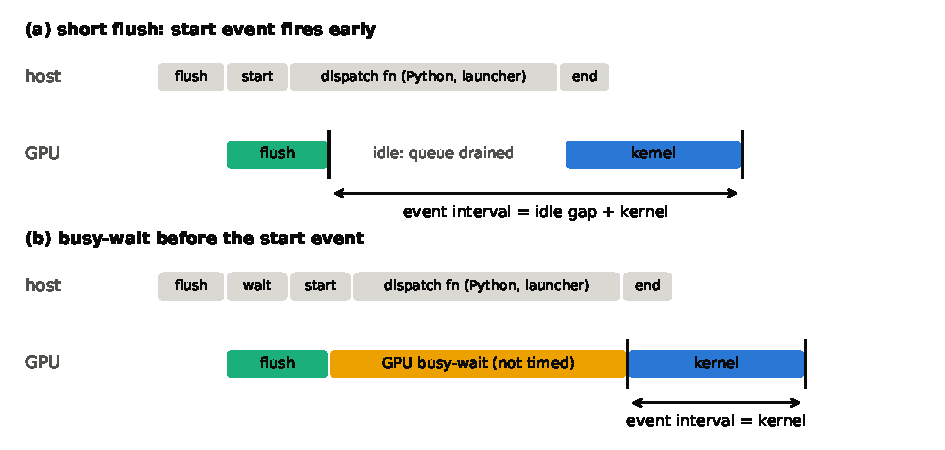
\includegraphics[width=0.92\textwidth]{fig_queue_drain.pdf}
\caption{Queue drain (schematic). (a) When the flush ends before the host has enqueued the kernel, the GPU reaches
the start event early and the event interval includes the idle gap. (b) A GPU busy-wait enqueued before the start
event keeps the queue busy; the busy-wait itself is not timed.}
\label{fig:queue}
\end{figure}
\label{pitfall-2-queue-drain}

This is a known property of CUDA-event timing: NVIDIA\textquotesingle s nvbench documents that the start event "may be recorded a
non-trivial amount of time before" the timed kernel is ready, and blocks the stream with a \texttt{blocking\_\allowbreak{}kernel} until
all work is queued; a 2023 Speechmatics post recommends a \texttt{torch.cuda.\_\allowbreak{}sleep} before the start event for the same
reason (\hyperref[related-work-and-credit]{\S{}14}). What we add is where it bites in practice: Python harnesses that flush before every call, once
the flush is shortened.

In the loop \texttt{flush();\ start.record();\ fn();\ end.record()}, the start event is timestamped when the GPU reaches it.
If the GPU has already finished the flush when the host enqueues the start event, the timestamp is taken at once,
and the interval includes the time the host still needs to dispatch \texttt{fn} (Python, the Triton launcher or
PyTorch\textquotesingle s dispatcher). A 256~MiB flush keeps the GPU busy for about 1~ms on the laptop GPU, which hides this; an
L2-sized flush takes 12-18~\ensuremath{\mu}s. To test this we inserted a GPU busy-wait of about 300~\ensuremath{\mu}s
(\texttt{torch.cuda.\_\allowbreak{}sleep}) right before the start event. It runs before the start event and is not timed.

\textbf{Laptop GPU (host dispatch on WSL2: 72-139~\ensuremath{\mu}s).} Time relative to a 256~MiB read flush:

{\small
\begin{longtable}[]{@{}>{\raggedright\arraybackslash}p{(\linewidth - 6\tabcolsep) * \real{0.447}}>{\raggedright\arraybackslash}p{(\linewidth - 6\tabcolsep) * \real{0.183}}>{\raggedright\arraybackslash}p{(\linewidth - 6\tabcolsep) * \real{0.370}}@{}}
\toprule\noalign{}
Kernel, flush & do\_\allowbreak{}bench-style loop & with the busy-wait \\
\midrule\noalign{}
\endhead
\bottomrule\noalign{}
\endlastfoot
cuBLAS GEMV 12~MiB, L2-sized read & +66~\% & \textbf{0~\%} \\
Triton y = 2x (3~MiB), 2 \ensuremath{\times} L2 read & +167~\% & \textbf{0~\%} \\
Triton y = 2x, L2-sized \texttt{zero\_\allowbreak{}()} vs 256~MiB \texttt{zero\_\allowbreak{}()} (the Inductor setting) & +187~\% & \textbf{0~\%} \\
cuBLAS GEMV, \texttt{zero\_\allowbreak{}()} + 10~ms wait vs \texttt{zero\_\allowbreak{}()} & +348~\% & \textbf{+2.4~\%} \\
elementwise add 12~MiB, L2-sized read & +43~\% & +6.7~\% (the extra write-back of \hyperref[what-removes-the-residue-and-what-does-not]{\S{}6}) \\
\end{longtable}
}

\begin{itemize}
\tightlist
\item
  \textbf{The 256~MiB write and read flushes were unaffected by the busy-wait} (within 2.2~\%; also on the A100, RTX 5090
  and L40S hosts below): they already keep the queue busy.
\item
  \textbf{The real \texttt{do\_\allowbreak{}bench}, with \texttt{clear\_\allowbreak{}cache} patched:} the Triton kernel took 41-47~\ensuremath{\mu}s with an L2-sized read
  flush and 13.3~\ensuremath{\mu}s with the same flush followed by the busy-wait.
\end{itemize}

\textbf{Fast GPUs, new hosts.} Liger-Kernel RMSNorm on 16~MiB (the kernel behind the +164 to +537~\% numbers of the
nine-GPU study), L2-sized \texttt{zero\_\allowbreak{}()} relative to 256~MiB \texttt{zero\_\allowbreak{}()}; and a 16~MiB GEMV with no flush relative to a
256~MiB read flush. Host dispatch is the median host time to enqueue the RMSNorm; flush time is estimated as
L2 size over the DRAM rate of the 112~MiB GEMV.

{\small
\begin{longtable}[]{@{}>{\raggedright\arraybackslash}p{(\linewidth - 10\tabcolsep) * \real{0.267}}>{\raggedright\arraybackslash}p{(\linewidth - 10\tabcolsep) * \real{0.151}}>{\raggedright\arraybackslash}p{(\linewidth - 10\tabcolsep) * \real{0.160}}>{\raggedright\arraybackslash}p{(\linewidth - 10\tabcolsep) * \real{0.239}}>{\raggedright\arraybackslash}p{(\linewidth - 10\tabcolsep) * \real{0.184}}@{}}
\toprule\noalign{}
GPU & host dispatch & L2-sized flush (est.) & RMSNorm, L2-sized \texttt{zero\_\allowbreak{}()}: loop / busy-wait & GEMV 16~MiB, no flush \ensuremath{\div} read flush: loop / busy-wait \\
\midrule\noalign{}
\endhead
\bottomrule\noalign{}
\endlastfoot
A100-SXM4-40GB & 140~\ensuremath{\mu}s & \ensuremath{\approx} 37~\ensuremath{\mu}s & \textbf{+203~\% / \ensuremath{-}3~\%} & \textbf{1.50 / 0.76} \\
RTX 5090 & 43~\ensuremath{\mu}s & \ensuremath{\approx} 63~\ensuremath{\mu}s & 0~\% / \ensuremath{-}9~\% & 0.92 / 0.88 \\
L40S & 102~\ensuremath{\mu}s & \ensuremath{\approx} 138~\ensuremath{\mu}s & 0~\% / \ensuremath{-}1.5~\% & 0.93 / 0.93 \\
\end{longtable}
}

\begin{itemize}
\tightlist
\item
  \textbf{What it accounts for.} On the A100 host both anomalies of the nine-GPU study reproduced: the L2-sized write flush
  made the short kernel 3\ensuremath{\times} slower, and no flush was 1.5\ensuremath{\times} \emph{slower} than flushing (the failed check of \hyperref[negative-results-deviations-and-limitations]{\S{}13}). Both
  disappeared with the busy-wait, and no flush became faster, as it should. They are queue drain, not cache
  effects.
\item
  \textbf{They depend on the host, not only on the GPU.} On our RTX 5090 and L40S hosts the host dispatched faster than
  the L2-sized flush ran, and neither anomaly appeared. Across the four machines we measured (with the laptop),
  the inflation appeared exactly where host dispatch took longer than the flush; this rule was formed after seeing
  the data. The RTX 5090 host of the nine-GPU study did show +537~\%; its dispatch time was not recorded.
\item
  \textbf{Who is exposed.} Python harnesses with a short flush on a fast GPU: Inductor\textquotesingle s benchmarker (L2-sized buffer),
  any tool after shrinking its flush, and any loop with no flush. Inductor returns the minimum over samples, which
  our repro shows is less affected than the median. C++ harnesses (nvbench, CUTLASS) likely dispatch faster; we
  did not measure them.
\item
  \textbf{Related.} Helion\textquotesingle s autotuner (PR \#4126~\cite{helion4126}, merged 2026-10-23) found that for microsecond kernels its benchmarks
  "mostly timed the flush" and added flush regimes; that is a different mechanism with the same lesson, that the
  flush step can dominate short-kernel timings.
\end{itemize}

\section{Pitfall 3: who pays for a kernel\textquotesingle s own writes}\label{pitfall-3-who-pays-for-a-kernels-own-writes}

If a kernel\textquotesingle s output fits within the amount of dirty data the L2 holds (about half of it on the laptop GPU), the
output is still dirty in the L2 when the kernel ends. Under a read flush, that
write-back happens during the \emph{next} flush, outside any timed window. Counters on the laptop GPU (fraction of
the kernel\textquotesingle s own output written to DRAM inside its timed window, median of 15 calls):

{\small
\begin{longtable}[]{@{}>{\raggedright\arraybackslash}p{(\linewidth - 8\tabcolsep) * \real{0.368}}>{\raggedright\arraybackslash}p{(\linewidth - 8\tabcolsep) * \real{0.206}}>{\raggedright\arraybackslash}p{(\linewidth - 8\tabcolsep) * \real{0.290}}>{\raggedright\arraybackslash}p{(\linewidth - 8\tabcolsep) * \real{0.136}}@{}}
\toprule\noalign{}
Kernel (elementwise add) & read flush 256~MiB ("cold") & rotated input/output copies ("steady") & no flush \\
\midrule\noalign{}
\endhead
\bottomrule\noalign{}
\endlastfoot
output 0.125 \ensuremath{\times} L2 & \textbf{0.00} & \textbf{0.99} & 0.00 \\
output 2 \ensuremath{\times} L2 & 0.75 & 1.00 & 0.99 \\
\end{longtable}
}

\begin{itemize}
\tightlist
\item
  \textbf{On the laptop GPU, under a read flush, a kernel with an output below about L2/2 does not pay for writing it at
  all}; a large output pays for all but about L2/2, which equals the residue a long write stream leaves there
  (0.50 L2).
\item
  \textbf{Rotating over copies whose total footprint is \ensuremath{\ge} 4 \ensuremath{\times} L2 charges one output\textquotesingle s write-back per call}, which is
  what a steady stream of independent calls costs.
\item
  \textbf{In time} (laptop GPU, \texttt{cleanbench}): steady vs cold was +0.2~\% for the GEMV (tiny output), +14~\% for the
  2 \ensuremath{\times} L2 elementwise kernel (+6.4~\ensuremath{\mu}s, against an implied 5.7~\ensuremath{\mu}s to write 0.5 L2 at its DRAM rate) and +38~\% for a
  0.4 \ensuremath{\times} L2 elementwise kernel (+3.7~\ensuremath{\mu}s, against an implied 4.6~\ensuremath{\mu}s).
\item
  \textbf{On large-L2 GPUs (new hosts)} steady vs cold was, for an elementwise kernel with a 0.25 \ensuremath{\times} L2 output, +39~\%
  (A100), +67~\% (RTX 5090) and +109~\% (L40S); for the 112~MiB GEMV within \ensuremath{\pm}1.1~\%; for a Liger RMSNorm with a
  64~MiB output +16~\%, +10~\% and +72~\%. The long-stream residue implied by \hyperref[how-big-is-the-bias-nine-gpus]{\S{}5} predicted the first two RMSNorm
  values within 0.006 but under-predicted L40S 2.5-fold: there, even a 0.67 \ensuremath{\times} L2 output was almost entirely
  untimed in cold mode.
\item
  \textbf{Prior art.} We have not found this corollary stated. The nearest is a question on NVIDIA\textquotesingle s developer forum
  (2026-10-03) noting that Nsight Compute\textquotesingle s \texttt{-\/-cache-control\ all} leaves no flush write-back and asking for a
  "dirty" mode, because "real world scenario usually start with L2 dirty from the previous kernel".
\item
  \textbf{Neither number is "the" time of the kernel in a model.} If the next operation reads or overwrites the output
  while it is still in L2, the write-back may never happen. Cold and steady are two measurement conditions, not
  guaranteed bounds: cold leaves part of the kernel\textquotesingle s own write-back out, steady charges one earlier call\textquotesingle s. Kernels that write different amounts (fused vs unfused, or a kernel
  that writes an intermediate) are compared fairly only if both numbers are reported.
\end{itemize}

\section{End-to-end check: which number predicts a decode step?}\label{end-to-end-check-which-number-predicts-a-decode-step}

For workload optimization, a per-kernel time is useful if it predicts what the kernel costs inside the workload. We
built a decode proxy: four layers
of Llama-2-7B shapes (hidden 4096, FFN 11008) at batch 1, each running its four weight GEMVs (fused QKV, O, fused
gate+up, down) with its own weights, in fp16 (cuBLAS), int4 (tinygemm) and NF4 (bitsandbytes). The whole step was
captured in one CUDA graph and replayed back to back, as decode loops do; its median time is the reference. Each
harness\textquotesingle s per-kernel times were summed over the step and compared with it (pre-registered; five GPUs).

{\small
\begin{longtable}[]{@{}>{\raggedright\arraybackslash}p{(\linewidth - 10\tabcolsep) * \real{0.210}}>{\raggedright\arraybackslash}p{(\linewidth - 10\tabcolsep) * \real{0.093}}>{\raggedright\arraybackslash}p{(\linewidth - 10\tabcolsep) * \real{0.224}}>{\raggedright\arraybackslash}p{(\linewidth - 10\tabcolsep) * \real{0.237}}>{\raggedright\arraybackslash}p{(\linewidth - 10\tabcolsep) * \real{0.237}}@{}}
\toprule\noalign{}
GPU & L2 & fp16 step: shipped / cold & int4 step: shipped / cold & int4 speedup error: shipped / cold \\
\midrule\noalign{}
\endhead
\bottomrule\noalign{}
\endlastfoot
RTX 3060 Laptop & 3~MiB & +5.2~\% / +2.0~\% & +8.6~\% / +1.8~\% & \ensuremath{-}3.1~\% / +0.2~\% \\
RTX 4060 & 24~MiB & +8.2~\% / +0.6~\% & \textbf{+43.6~\%} / +2.0~\% & \textbf{\ensuremath{-}24.6~\%} / \ensuremath{-}1.4~\% \\
A100-SXM4-40GB & 40~MiB & \textbf{+26.3~\%} / +5.2~\% & \textbf{+46.2~\%} / +17.5~\% & \ensuremath{-}13.6~\% / \ensuremath{-}10.4~\% \\
H100 NVL & 60~MiB & \textbf{+32.4~\%} / +8.4~\% & +22.6~\% / +17.2~\% & +8.0~\% / \ensuremath{-}7.5~\% \\
L40S & 96~MiB & \textbf{+28.1~\%} / +2.0~\% & \textbf{+52.5~\%} / +7.1~\% & \ensuremath{-}16.1~\% / \ensuremath{-}4.8~\% \\
\end{longtable}
}

\begin{itemize}
\tightlist
\item
  \textbf{The shipped write flush over-predicts the step} on every GPU with \ensuremath{\ge} 40~MiB of L2, by 26-32~\% for fp16 and
  23-53~\% for int4.
\item
  \textbf{It also ranks kernels wrongly.} On the RTX 4060, summed shipped times put NF4 ahead of tinygemm; in the step,
  tinygemm is 15~\% faster, and the read-flush times rank them correctly. On the H100 NVL, the step\textquotesingle s NF4 speedup over
  fp16 is 1.14\ensuremath{\times}; the shipped times predict 1.32\ensuremath{\times}, the read-flush times 1.09\ensuremath{\times}.
\item
  \textbf{The read flush with a busy-wait ("cold") is close on the consumer GPUs and the L40S} (within 2~\% for fp16 and
  2-7~\% for int4), \textbf{but not on the A100 and H100}: 5-8~\% for fp16 and 17~\% for int4, against our pre-registered
  10~\%. There an int4 GEMV takes 18-28~\ensuremath{\mu}s, and event timing adds a fixed per-call cost that graph replay does not
  (2.2-3.4~\ensuremath{\mu}s per call on the rented RTX 4060 and A100 hosts of \hyperref[kernel-by-kernel-does-a-single-kernel-benchmark-match-the-same-kernel-inside-the-decode-proxy]{\S{}9.1}; the H100 was not re-measured).
\item
  \textbf{Limitations.} The proxy has only GEMVs (no attention, norms or activations). NF4 was mispredicted by every
  harness on the L40S (cold +36~\%; cause unknown).
\end{itemize}

\textbf{Can a per-kernel time get within 1~\%?} The cold time\textquotesingle s excess over the step was 2-5~\ensuremath{\mu}s per kernel on every GPU,
which suggests a fixed per-kernel cost of event timing rather than a cache effect. We therefore timed each kernel the
way the step runs it: one CUDA graph calling the kernel once per weight copy (copies covering \ensuremath{\ge} 4 \ensuremath{\times} L2, so every call
is cold), replayed back to back, divided by the number of calls (pre-registered; the A100 host was the one used in
B19 and B21, the H100 NVL host was new):

{\small
\begin{longtable}[]{@{}>{\raggedright\arraybackslash}p{(\linewidth - 10\tabcolsep) * \real{0.192}}>{\raggedright\arraybackslash}p{(\linewidth - 10\tabcolsep) * \real{0.217}}>{\raggedright\arraybackslash}p{(\linewidth - 10\tabcolsep) * \real{0.205}}>{\raggedright\arraybackslash}p{(\linewidth - 10\tabcolsep) * \real{0.217}}>{\raggedright\arraybackslash}p{(\linewidth - 10\tabcolsep) * \real{0.169}}@{}}
\toprule\noalign{}
GPU & step error, fp16 / int4: graph-batched & cold & shipped & int4 speedup error: graph-batched \\
\midrule\noalign{}
\endhead
\bottomrule\noalign{}
\endlastfoot
A100-SXM4-40GB & \textbf{+1.0~\% / +1.6~\%} & +6.0~\% / +17.5~\% & +26.9~\% / +47.1~\% & \textbf{\ensuremath{-}0.6~\%} \\
H100 NVL & \ensuremath{-}12.2~\% / \ensuremath{-}19.5~\% & \ensuremath{-}4.5~\% / \ensuremath{-}6.4~\% & +16.8~\% / +0.5~\% & +9.1~\% \\
\end{longtable}
}

\begin{itemize}
\tightlist
\item
  \textbf{On the A100 host, close:} the step time within 1.0-1.6~\% (NF4 0.2~\%) and the int4 speedup within 0.6~\%.
\item
  \textbf{On the H100 NVL, no per-kernel method came within 5~\%.} The graph-batched time was 12-20~\% \emph{below} the step.
  Where 1~\% matters on such GPUs, time the model\textquotesingle s own graph.
\item
  \textbf{The decode proxy changed across hosts, while isolated-kernel times were stable.} The same H100 NVL step took
  532~\ensuremath{\mu}s on one rented host and
  616~\ensuremath{\mu}s on another (fp16 +16~\%, int4 +27~\%, NF4 +9~\%). The isolated kernels did not move: their cold times on the
  two hosts agreed within \ensuremath{-}0.8 to +4.3~\% (all 12 kernel rows), and the sum of the second host\textquotesingle s graph-batched times
  matched the \emph{first} host\textquotesingle s step within 2.4~\% (fp16 +1.7~\%, int4 +2.4~\%, NF4 \ensuremath{-}2.2~\%). So the H100 miss is a
  property of how the second host ran the 16-kernel step, not of per-kernel timing or of the chip (post hoc,
  two hosts, one run set each). The hosts differed in power limit (400~W vs 300~W), driver (580.178 vs 615.71) and
  virtualization (VM pass-through vs unreported); we did not log clocks or throttle reasons during the step, so we
  cannot attribute the difference. The A100 runs of \hyperref[end-to-end-check-which-number-predicts-a-decode-step]{\S{}9} (B21 and B22) used one host, so the A100 1~\% result is also
  from one host.
\end{itemize}

\subsection{Kernel by kernel: does a single-kernel benchmark match the same kernel inside the decode proxy?}

\begin{figure}[tbp]
\centering
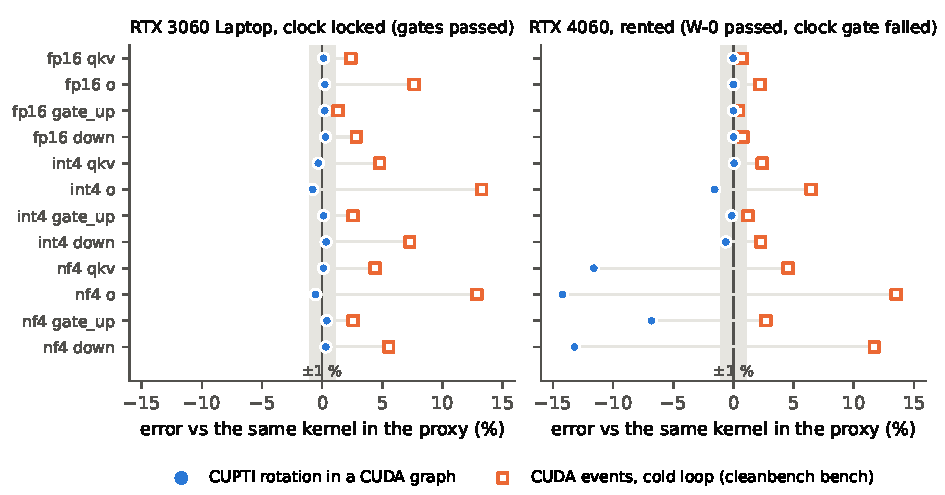
\includegraphics[width=0.95\textwidth]{fig_kernel_errors.pdf}
\caption{Per-kernel error against the same kernel inside the GEMV-only decode proxy (ratio of medians over three
runs; shaded band $\pm$1\,\%). Left: laptop GPU with the SM clock locked, all gates passed. Right: rented RTX 4060,
clock not locked (power-capped); the NF4 rows show a context effect of unknown cause.}
\label{fig:errors}
\end{figure}
\label{kernel-by-kernel-does-a-single-kernel-benchmark-match-the-same-kernel-inside-the-decode-proxy}

Sums over a step can hide errors that cancel. We therefore compared each kernel\textquotesingle s benchmark time with the same
kernel\textquotesingle s time inside the decode step (pre-registered):

\begin{itemize}
\tightlist
\item
  \textbf{Reference.} The step\textquotesingle s CUDA graph, replayed back to back after at least 1 s of sustained replays; each kernel\textquotesingle s
  duration from CUPTI activity records (the GPU\textquotesingle s own start and end timestamps), 4 layers \ensuremath{\times} 300 replays.
\item
  \textbf{Harnesses} on the same kernels:

  \begin{itemize}
  \tightlist
  \item
    \emph{CUPTI rotation}: CUPTI durations over a CUDA graph that calls the kernel once per weight copy (copies \ensuremath{\ge} 4 \ensuremath{\times} L2,
    as in \hyperref[end-to-end-check-which-number-predicts-a-decode-step]{\S{}9}), after the same warm-up;
  \item
    the same after 1 s of idle GPU and no warm-up;
  \item
    \texttt{cleanbench}\textquotesingle s cold loop (read flush, busy-wait) timed by CUPTI;
  \item
    \texttt{cleanbench} cold as in \hyperref[end-to-end-check-which-number-predicts-a-decode-step]{\S{}9} (CUDA events);
  \item
    the graph-batched event time of \hyperref[end-to-end-check-which-number-predicts-a-decode-step]{\S{}9}.
  \end{itemize}
\item
  \textbf{Interleaving.} The reference and CUPTI rotation were measured in three alternating rounds per run, so slow
  drift affects both; three runs per GPU.
\item
  \textbf{Gates.} Tracing must not change the step\textquotesingle s CUDA-event time by more than 0.5~\%; the reference must be stable
  (IQR \ensuremath{\le} 5~\% of the median); every trace segment must hold exactly the expected kernels. After the first laptop run
  failed, an amendment (locked before the next run) added a clock gate: the SM clock within \ensuremath{\pm}1~\% of its median in
  \ensuremath{\ge} 99~\% of busy samples, and no thermal or hardware slowdown in the driver\textquotesingle s counters.
\end{itemize}

{\small
\begin{longtable}[]{@{}>{\raggedright\arraybackslash}p{(\linewidth - 6\tabcolsep) * \real{0.569}}>{\raggedright\arraybackslash}p{(\linewidth - 6\tabcolsep) * \real{0.295}}>{\raggedright\arraybackslash}p{(\linewidth - 6\tabcolsep) * \real{0.136}}@{}}
\toprule\noalign{}
RTX 3060 Laptop, SM clock locked at 1,000~MHz (observed 1,005) & Error vs the same kernel in the step (12 kernels) & Within 1~\% \\
\midrule\noalign{}
\endhead
\bottomrule\noalign{}
\endlastfoot
CUPTI rotation, 1 s warm-up & \textbf{\ensuremath{-}0.79 to +0.39~\%} & \textbf{12/12} \\
CUPTI rotation, after 1 s idle & \ensuremath{-}1.6 to +0.9~\% & 10/12 \\
Graph-batched CUDA events (\hyperref[end-to-end-check-which-number-predicts-a-decode-step]{\S{}9}) & 0.0 to +2.4~\% & 6/12 \\
CUPTI, \texttt{cleanbench} cold loop & \ensuremath{-}2.0 to +3.4~\% & 1/12 \\
CUDA events, \texttt{cleanbench} cold loop & +1.3 to +13.3~\% & 0/12 \\
\end{longtable}
}

The error of a harness is
\[E = \frac{\tilde{t}_{\mathrm{harness}}}{\tilde{t}_{\mathrm{proxy}}} - 1,\]
where \(\tilde{t}\) is the median over three runs of each run\textquotesingle s median kernel time, in the harness and inside the proxy.
All gates passed
and every pre-registered prediction for this run held. The kernels took 49-645~\ensuremath{\mu}s. Unaggregated, the per-run errors
were within 0.86~\% (36 of 36 kernel-runs), and the errors of the paired rounds (reference and harness measured back
to back, 108 pairs) had a median of 0.30~\%, a 95th percentile of 0.95~\% and a maximum of 1.10~\% (104 of 108 within
1~\%). On the RTX 4060 below, the paired-round 95th percentile was 13.8~\%.

\begin{itemize}
\tightlist
\item
  \textbf{What was needed.}

  \begin{itemize}
  \tightlist
  \item
    \emph{The GPU\textquotesingle s timestamps instead of events.} On the two rented hosts, event-bracketed intervals exceeded the CUPTI
    kernel durations in the same cold loop by 2.2-3.4~\ensuremath{\mu}s per call (3-22~\ensuremath{\mu}s on the laptop under WSL2). The excess
    includes launch latency and idle gaps inside the event interval, not only the cost of the events themselves.
  \item
    \emph{Rotation inside a graph instead of a flush.} The cold loop was 1-3~\% off even when timed by CUPTI: it differs
    from the step in cache state and context, not only in the timer.
  \item
    \emph{Interleaving.} Even with the clock locked, the reference moved 1.2-2.2~\% between rounds.
  \item
    \emph{A steady clock.} The unlocked laptop run failed its gates: the GPU reached 87 \ensuremath{^\circ}C, the SM clock ranged
    1,005-1,747~MHz, and the driver\textquotesingle s thermal-slowdown counter rose by 53 s. Between rounds, the in-step time of the
    fp16 kernels moved 2-3~\%, that of the int4 and NF4 kernels 27-30~\%.
  \end{itemize}
\item
  \textbf{Rented hosts refused clock locking} ("The current user does not have permission to change clocks"), as we
  predicted.

  \begin{itemize}
  \tightlist
  \item
    \textbf{RTX 4060:} the pre-registered gates and the thermal check passed, but the clock gate did not: the clock was not steady
    (2,355-2,805~MHz; power-capped in 130 of 202 busy samples). CUPTI rotation was within 0.02~\% for fp16 and 1.6~\% for int4, but 6.8-14.2~\% \emph{below} the step for
    NF4 (bitsandbytes), with similar clocks in both phases (medians 2,535 and 2,573~MHz): this kernel ran faster
    when repeated than among other kernels (cause unknown). Events in the cold loop: +0.4 to +13.5~\%.
  \item
    \textbf{A100-SXM4:} the tracing gate failed (CUPTI added 1.0-2.2~\% to the step, whose kernels took 14-138~\ensuremath{\mu}s), so
    this run is descriptive only: CUPTI rotation \ensuremath{-}4.1 to +3.7~\%, events in the cold loop +3.0 to +22.2~\%. The clock
    was power-capped (1,260-1,410~MHz).
  \item
    The RTX 4090 and H100 NVL hosts never became reachable and were destroyed unused.
  \end{itemize}
\item
  \textbf{Clock sensitivity (post hoc).} A two-term frequency-scaling model, \(t(f) = a/f + b\), splits a kernel\textquotesingle s time into
  a part that scales with the SM clock \(f\) and a part that does not (DRAM at a fixed memory clock). With
  \(s = (a/f_0)/t(f_0)\), a change of the clock from \(f_0\) to \(f_1\) changes the time by
  \[\frac{t(f_1)}{t(f_0)} - 1 = s\left(\frac{f_0}{f_1} - 1\right) \approx -s\,\frac{\Delta f}{f}, \qquad 0 \le s \le 1,\]
  so it is at most \(f_0/f_1 - 1\) (a 20~\% clock drop can add up to 25~\%). From the laptop\textquotesingle s unlocked
  and locked runs (\texttt{clock\_\allowbreak{}sensitivity.py}; the unlocked clock summarized from 13-22 one-second \texttt{nvidia-smi} samples
  per variant, as a median or a mean): s = 0.00-0.04 for the fp16 GEMVs, 0.79-0.91 for int4 and 0.61-0.66 for NF4.
  Two clock states determine the two parameters exactly, so this is a rough estimate, not a validated model. It is
  consistent, on the laptop, with fp16 timing withstanding clock changes and int4 / NF4 not, and it makes the clock
  an unlikely cause of the RTX 4060\textquotesingle s NF4 gap (whose s we did not measure). Richer GPU frequency-scaling models exist
  (e.g. CRISP, \hyperref[related-work-and-credit]{\S{}14}); we have not tested a correction based on this one.
\end{itemize}

\section{cleanbench}\label{cleanbench}

\texttt{cleanbench.py} (one file, PyTorch and Triton) times a callable with:

\begin{itemize}
\tightlist
\item
  a \textbf{read flush} (the PR \#12556~\cite{tr12556} kernel) over a buffer of max(256~MiB, 4 \ensuremath{\times} L2), cached per device;
\item
  a \textbf{GPU busy-wait} before every start event, sized min(5~ms, max(100~\ensuremath{\mu}s, 3 \ensuremath{\times} the measured host dispatch time)), a
  simpler, fixed-length stand-in for nvbench\textquotesingle s blocking kernel;
\item
  \texttt{mode="cold"} (flush before every call) or \texttt{mode="steady"} (no flush; the caller passes callables over copies,
  whose total footprint should be \ensuremath{\ge} 4 \ensuremath{\times} L2, and the harness rotates over them);
\item
  median, mean, IQR, p95, and warnings when the median is within 30 timer ticks (\ensuremath{\approx} 1.02~\ensuremath{\mu}s each) and most samples
  fall on the tick grid, when the IQR exceeds 10~\% of the median, and, in cold mode, that the kernel\textquotesingle s own
  write-back is partly untimed.
\end{itemize}

\begin{codebox}
\begin{Verbatim}[fontsize=\small]
import cleanbench as cb
cold = cb.bench(lambda: f(x, y))                       # read flush + busy-wait
rot = [lambda i=i: f(xs[i], ys[i]) for i in range(n)]  # copies covering >= 4 x L2
steady = cb.bench(rotate=rot, mode="steady")
print(cold.median_us, steady.median_us, cold.warnings)
\end{Verbatim}
\end{codebox}

\textbf{Validation on the laptop GPU} (per cell, 15 \texttt{bench()} calls of 100 timed calls each over 3 runs; value = median
over the calls of each call\textquotesingle s mean; the \texttt{do\_\allowbreak{}bench} column compares \texttt{do\_\allowbreak{}bench}\textquotesingle s median with that value):

{\small
\begin{longtable}[]{@{}>{\raggedright\arraybackslash}p{(\linewidth - 8\tabcolsep) * \real{0.469}}>{\raggedright\arraybackslash}p{(\linewidth - 8\tabcolsep) * \real{0.186}}>{\raggedright\arraybackslash}p{(\linewidth - 8\tabcolsep) * \real{0.144}}>{\raggedright\arraybackslash}p{(\linewidth - 8\tabcolsep) * \real{0.202}}@{}}
\toprule\noalign{}
Kernel & cold, 2 \ensuremath{\times} L2 flush vs 256~MiB & steady vs cold & shipped \texttt{do\_\allowbreak{}bench} vs cold \\
\midrule\noalign{}
\endhead
\bottomrule\noalign{}
\endlastfoot
cuBLAS GEMV 12~MiB & \ensuremath{-}0.05~\% & +0.2~\% & +12~\% \\
elementwise add, 2 \ensuremath{\times} L2 & +1.6~\% & +14~\% & +15~\% \\
elementwise add, 0.4 \ensuremath{\times} L2 & +5.6~\% & +38~\% & +36~\% \\
Triton y = 2x, 0.5 \ensuremath{\times} L2 & +9.4~\% & +46~\% & +41~\% \\
\end{longtable}
}

The first column is why the default buffer is not 2 \ensuremath{\times} L2. On the A100, RTX 5090 and L40S hosts, the shipped
\texttt{do\_\allowbreak{}bench} read +16~\%, +11~\% and +25~\% above \texttt{cleanbench}\textquotesingle s cold time for the 112~MiB GEMV, matching the nine-GPU
study\textquotesingle s +16.0~\%, +10.8~\% and +25.3~\%, measured on different hosts against a different baseline.

\textbf{Kernel time from the GPU\textquotesingle s timestamps (\texttt{bench\_\allowbreak{}graph}, \texttt{compare}).} \texttt{bench\_\allowbreak{}graph(rotate)} captures callables over
input copies (\ensuremath{\ge} 4 \ensuremath{\times} L2 in total) in one CUDA graph, keeps the GPU busy for at least 1 s, and reads each call\textquotesingle s
kernel durations from CUPTI; \texttt{compare} times several candidates in interleaved rounds, in a seeded random order per
round. \texttt{locked\_\allowbreak{}sm\_\allowbreak{}clock(mhz)} locks the SM clock where permitted (root or Administrator) and always resets it.
\texttt{Result.quality} reports checks for exact CUPTI records, a tracing effect \ensuremath{\le} 0.5~\% (traced and untraced replays are
both timed), readable clock-event counters that did not grow, and inputs covering \ensuremath{\ge} 4 \ensuremath{\times} L2 (\texttt{footprint\_\allowbreak{}bytes}).
The \texttt{validated} flag indicates that these checks passed; otherwise the result is labelled exploratory. It does
not establish the clock-stability condition used in \hyperref[kernel-by-kernel-does-a-single-kernel-benchmark-match-the-same-kernel-inside-the-decode-proxy]{\S{}9.1} or guarantee 1~\% agreement with the workload. The counters
catch throttling, not every small boost step; 1~\% agreement was demonstrated separately on one GPU with a locked
clock (\hyperref[kernel-by-kernel-does-a-single-kernel-benchmark-match-the-same-kernel-inside-the-decode-proxy]{\S{}9.1}). Each callable must run on the current stream without overlapping kernels.

\textbf{Limitations.} \texttt{torch.cuda.\_\allowbreak{}sleep} is a private PyTorch API. Steady mode and \texttt{bench\_\allowbreak{}graph} need the caller to build
input/output copies. With CUDA events (\texttt{bench}), kernels shorter than about 30~\ensuremath{\mu}s remain limited by the timer\textquotesingle s
\ensuremath{\approx} 1~\ensuremath{\mu}s resolution. \texttt{bench\_\allowbreak{}graph} reached 1~\% only with a locked clock, on one GPU (\hyperref[kernel-by-kernel-does-a-single-kernel-benchmark-match-the-same-kernel-inside-the-decode-proxy]{\S{}9.1}), and CUPTI tracing itself
added 1-2~\% on an A100.

\section{Measurement pitfall: per-kernel DRAM write counters lose bytes}\label{measurement-pitfall-per-kernel-dram-write-counters-lose-bytes}

We ran a kernel writing w \ensuremath{\times} L2, followed by a flush. One range enclosing both counts \ensuremath{\approx} 100~\% of the written
bytes. The sum of per-kernel \texttt{dram\_\allowbreak{}\_\allowbreak{}bytes\_\allowbreak{}write.sum} does not; the share of the written bytes it loses:

{\small
\begin{longtable}[]{@{}l@{\hspace{1.6em}}r@{\hspace{1.6em}}r@{\hspace{1.6em}}r@{}}
\toprule\noalign{}
Die (GPU, L2) & w = 0.75 L2 & w = 1.0 L2 & w = 1.5 L2 \\
\midrule\noalign{}
\endhead
\bottomrule\noalign{}
\endlastfoot
GA106 (RTX 3060 Laptop, 3~MiB) & 8.9~\% & 6.7~\% & 0.1~\% \\
GA102 (RTX 3090, 6~MiB) & 14.4~\% & 9.2~\% & 3.5~\% \\
TU106 (RTX 2060 SUPER, 4~MiB) & 14.7~\% & 16.9~\% & 5.7~\% \\
AD103 (RTX 4080 SUPER, 64~MiB) & 5.8~\% & 4.9~\% & 3.2~\% \\
\end{longtable}
}

\begin{itemize}
\tightlist
\item
  \textbf{Per-kernel attribution misses them.} Two back-to-back ranges also lose bytes: 4-9~\% on GA102, 5-13~\% on TU106
  and 1-2~\% on AD103. All with \texttt{-\/-cache-control\ none}, Nsight Compute 2024.2.1.
\item
  \textbf{Still present in the latest release, on GA106.} Re-run on GA106 with Nsight Compute 2026.4.0 (newest in NVIDIA\textquotesingle s package
  repository on 2026-11-06), back to back with 2024.2.1: 8.1~\% / 5.4~\% / 0.2~\% lost at w = 0.75 / 1.0 / 1.5 L2, against
  8.6~\% / 5.8~\% / 0.2~\% with 2024.2.1 in the same session (pre-registered: "persists").
\item
  \textbf{Not yet measured on A100/H100.} The other three dies were measured with 2024.2.1 only. One attempt with Nsight Compute
  2025.2.1 on an RTX 5060 Ti returned n/a for the DRAM metrics.
\item
  \textbf{The dirty threshold behind \hyperref[background]{\S{}2}}, write-back fraction at a dirty footprint of 0.4375 / 0.625 L2: GA106 (3~MiB)
  0.014 / 0.991; GA102 (6~MiB) 0.009 / 0.974; TU106 (4~MiB) 0.016 / 0.976; AD103 (64~MiB) 0.071 / 0.933.
\end{itemize}

\section{Recommendations for tool authors}\label{recommendations-for-tool-authors}

\begin{itemize}
\tightlist
\item
  \textbf{Triton \texttt{do\_\allowbreak{}bench}:} PR \#12556~\cite{tr12556} would remove pitfall 1. Its 256~MiB buffer already avoided pitfall 2 on the four
  machines where we tested it with a busy-wait; a busy-wait after the flush would make that independent of GPU and
  host speed.
\item
  \textbf{PyTorch Inductor:} switching \texttt{zero\_\allowbreak{}()} to a read on the existing L2-sized buffer is not enough: it leaves the
  previous call\textquotesingle s output partly dirty (\hyperref[what-removes-the-residue-and-what-does-not]{\S{}6}) and lets the queue drain on fast GPUs (\hyperref[pitfall-2-queue-drain]{\S{}7}). Use a sufficiently large
  read buffer to reduce the previous call\textquotesingle s dirty output residue, and keep the GPU busy before the start event to
  prevent queue drain. Our conservative default uses max(256~MiB, 4 \ensuremath{\times} L2) plus a GPU busy-wait.
\item
  \textbf{nvbench, CUTLASS:} a read kernel instead of the memset (or a read pass after it).
\item
  \textbf{Leaderboards and LLM-kernel evaluations (KernelBench, GPU MODE):} state the flush method; consider reporting a
  steady-state time, since generated kernels differ in how much they write.
\item
  \textbf{All tools, when per-kernel numbers should match a model:} consider CUPTI durations over a CUDA graph that rotates
  inputs, with a warm-up and interleaved candidates, and report whether tracing, clock and footprint conditions held
  (\hyperref[kernel-by-kernel-does-a-single-kernel-benchmark-match-the-same-kernel-inside-the-decode-proxy]{\S{}9.1}); where they do not, time the model\textquotesingle s graph. Record the SM clock and the driver\textquotesingle s clock-event counters with
  every result.
\end{itemize}

\textbf{Observed timing hazards} (from this report; the rows measure different quantities under different conditions,
overlap, and are not additive):

{\small
\begin{longtable}[]{@{}>{\raggedright\arraybackslash}p{(\linewidth - 8\tabcolsep) * \real{0.225}}>{\raggedright\arraybackslash}p{(\linewidth - 8\tabcolsep) * \real{0.189}}>{\raggedright\arraybackslash}p{(\linewidth - 8\tabcolsep) * \real{0.293}}>{\raggedright\arraybackslash}p{(\linewidth - 8\tabcolsep) * \real{0.293}}@{}}
\toprule\noalign{}
Hazard & What is distorted & Observed here (setting) & Remedy (status) \\
\midrule\noalign{}
\endhead
\bottomrule\noalign{}
\endlastfoot
Write flush (dirty L2) & isolated cold time & +6.6 to +25.3~\% (decode GEMV, nine GPUs) & read flush (validated with counters on one GPU, timing on nine) \\
Queue drain & isolated cold time & up to +203~\% (short kernel, A100 host) & busy-wait before the start event (rescued on two hosts) \\
Own write-back untimed & cold vs stream of calls & up to about L2/2 of the output (laptop counters) & also report steady state (\hyperref[pitfall-3-who-pays-for-a-kernels-own-writes]{\S{}8}) \\
Event interval vs kernel duration & per-call time & 2.2-3.4~\ensuremath{\mu}s per call (two rented hosts) & CUPTI durations (\hyperref[kernel-by-kernel-does-a-single-kernel-benchmark-match-the-same-kernel-inside-the-decode-proxy]{\S{}9.1}) \\
Cold loop vs the proxy\textquotesingle s context & per-kernel time in the proxy & 1-3~\% (laptop, locked clock) & rotation inside a CUDA graph (one GPU) \\
SM clock changes & any time & 27-30~\% between rounds for int4 / NF4 (unlocked laptop) & lock the clock, or report the change (\hyperref[kernel-by-kernel-does-a-single-kernel-benchmark-match-the-same-kernel-inside-the-decode-proxy]{\S{}9.1}) \\
CUPTI tracing & traced vs untraced graph & 0.03-2.2~\% of the proxy step, up to 3.7~\% of a rotation graph (A100) & check tracing on vs off (\hyperref[kernel-by-kernel-does-a-single-kernel-benchmark-match-the-same-kernel-inside-the-decode-proxy]{\S{}9.1}) \\
Kernel context (NF4, RTX 4060) & per-kernel time in the proxy & up to 14~\% & time the model\textquotesingle s graph (cause unknown) \\
Host (same GPU model) & absolute step time & 9-27~\% (two H100 NVL hosts) & tune on the deployment host (cause unknown) \\
\end{longtable}
}

\section{Negative results, deviations and limitations}\label{negative-results-deviations-and-limitations}

\textbf{Wrong or partly wrong predictions} (all pre-registered):

\begin{itemize}
\tightlist
\item
  An L2-sized read flush evicted even a 24~KiB kernel\textquotesingle s inputs; we predicted it would leave them warm.
\item
  The busy-wait removed the inflation for two of three kernels; for the third, 6.7~\% remained, which matches, after
  the fact, the +6.6~\% implied by the extra write-back the counters measured; the locked rule scored "partial".
\item
  We predicted that waiting after a write flush slows timing through lower clocks; the busy-wait showed it is
  queue drain.
\item
  We predicted \texttt{cleanbench}\textquotesingle s cold time would not depend on the flush buffer between 2 \ensuremath{\times} L2 and 256~MiB; it does
  for short kernels with outputs of 0.4-0.5 L2.
\item
  In the nine-GPU study, we predicted only mild distortions of int4 speedups and marginal effects on GPUs with
  \ensuremath{\le} 32~MiB of L2; the RTX 4060 / 4060 Ti speedups moved by \ensuremath{-}23 to \ensuremath{-}24~\% and every kernel family was affected there.
\item
  Earlier: cache models (LRU plus dirty cap) did not predict single-kernel write-back on TU106/AD103 or the residue
  after long write streams; a "bandwidth slack absorbs the write-back" hypothesis passed only through a
  weight-format confound; an L2-sized write flush was not more biased than the 256~MiB one for the large GEMV.
\item
  For graph-batched timing (\hyperref[end-to-end-check-which-number-predicts-a-decode-step]{\S{}9}) we predicted the step within 2~\% on the A100 and H100; the A100 was within 1.6~\%, the
  H100 NVL 12-20~\% off. Two attempts on the laptop GPU failed the stability gate because another program was using
  the GPU.
\item
  In the end-to-end check (\hyperref[end-to-end-check-which-number-predicts-a-decode-step]{\S{}9}) we predicted the read flush with a busy-wait would come within 10~\% of the decode
  step on all five GPUs and predict the int4 speedup within 5~\% on the three with \ensuremath{\ge} 40~MiB of L2; on the A100 and
  H100 it missed the int4 step by 17~\% and the speedup by 8-10~\%.
\item
  In the per-kernel check (\hyperref[kernel-by-kernel-does-a-single-kernel-benchmark-match-the-same-kernel-inside-the-decode-proxy]{\S{}9.1}) we predicted that the gates would pass on rented hosts (the A100 failed the tracing
  gate), that the A100\textquotesingle s clock would be steady (it was power-capped) and that every kernel on the RTX 4060 would be
  within 1~\% (NF4 was 7-14~\% off). For the unlocked laptop run we had flagged the gates as at risk and made no
  accuracy prediction; it failed on thermal slowdown.
\item
  On fast GPUs we predicted that the L2-sized-flush anomaly would reproduce on the RTX 5090 (not on this host);
  that a 16~MiB GEMV would run \ensuremath{\ge} 15~\% faster with no flush than with a read flush once the queue is busy (A100
  yes; RTX 5090 12~\%, L40S 7~\%); and that the long-stream residue would predict the cold/steady gap of the 64~MiB
  RMSNorm on at least 3 of 4 GPUs (2 of the 3 measured; L40S off 2.5-fold; H100 not measured).
\end{itemize}

\textbf{Deviation.} In the nine-GPU study, our pre-registered check that the read flush evicts (no flush \ensuremath{\ge} 1.2\ensuremath{\times} faster
on 32~MiB of weights) failed on all four GPUs with L2 \ensuremath{\ge} 64~MiB; we replaced it after seeing one GPU with "the read
flush leaves the kernel at least as cold as \texttt{torch.sum}", validated earlier with counters. On an A100 host we
later reproduced the failed check (no flush 1.5\ensuremath{\times} slower than a read flush) and reversed it with a GPU busy-wait
(0.76\ensuremath{\times}): queue drain, not eviction, had made "no flush" look slow (\hyperref[pitfall-2-queue-drain]{\S{}7}).

\textbf{Deviations in \hyperref[kernel-by-kernel-does-a-single-kernel-benchmark-match-the-same-kernel-inside-the-decode-proxy]{\S{}9.1}.} The clock-locked laptop run is an amendment written after the unlocked run had failed its
gates; its predictions were locked before it ran. The rented runs added a clock-lock attempt in a wrapper script;
the measurement code and the rules were unchanged, and the clock-gate script was changed to make the locked clock
optional.

\textbf{Limitations.}

\begin{itemize}
\tightlist
\item
  No full-model measurement: the reference in \hyperref[end-to-end-check-which-number-predicts-a-decode-step]{\S{}9} is a four-layer, GEMV-only decode proxy, and the report is about
  what harnesses time, not about model throughput.
\item
  The 1~\% per-kernel result (\hyperref[kernel-by-kernel-does-a-single-kernel-benchmark-match-the-same-kernel-inside-the-decode-proxy]{\S{}9.1}) comes from one laptop GPU with a locked clock and kernels of 49-645~\ensuremath{\mu}s, against a
  GEMV-only proxy; on rented data-center GPUs we could not lock the clock and did not reach 1~\%.
\item
  The tool survey (\hyperref[who-is-affected-a-survey-of-15-benchmarking-tools]{\S{}3}) is a selection of commonly used tools, read once for eight of them.
\item
  One host per GPU model in the nine-GPU study (two for the RTX 4080 SUPER; the A100, RTX 5090 and L40S were
  re-measured on new hosts), rented containers with unlocked clocks, Triton 3.3.1 and torch 2.7.1.
\item
  Counter results (\hyperref[what-removes-the-residue-and-what-does-not]{\S{}6}, \hyperref[pitfall-3-who-pays-for-a-kernels-own-writes]{\S{}8}, \hyperref[measurement-pitfall-per-kernel-dram-write-counters-lose-bytes]{\S{}11}) come from one laptop GPU (\hyperref[what-removes-the-residue-and-what-does-not]{\S{}6}, \hyperref[pitfall-3-who-pays-for-a-kernels-own-writes]{\S{}8}) or four consumer dies (\hyperref[measurement-pitfall-per-kernel-dram-write-counters-lose-bytes]{\S{}11}); data-center L2
  policies may differ.
\item
  The host dispatch times on the laptop (WSL2) are longer than on a typical Linux server.
\end{itemize}

\section{Related work and credit}\label{related-work-and-credit}

\begin{itemize}
\tightlist
\item
  \textbf{Write-flush bias and the read flush:} reported in triton-lang/triton issue \#12554~\cite{tr12554} (2026-10-30), with Nsight
  Compute measurements on an A100 showing the write-back saturating at about half the L2 and kernels that read
  fewer bytes evicting fewer dirty lines; the read flush we use throughout is the kernel proposed in
  triton-lang/triton PR \#12556~\cite{tr12556} (measured there on an RTX 5090; open and awaiting maintainer review on 2026-11-06).
  PyTorch PR \#203681~\cite{pt203681} (open) addresses it for ROCm; TileOPs PR \#2822~\cite{tileops2822} and TileLang \#3534~\cite{tilelang3534} have switched to read
  flushes. Helion PR \#4126~\cite{helion4126} reworked its autotuner\textquotesingle s flush regimes for microsecond kernels. FlashInfer PR \#8076~\cite{fi8076} (open)
  proposes a read flush for its cold-L2 autotuning.
\item
  \textbf{Dirty L2 state:} deepseek-ai/DeepEP-Ascend issue \#17~\cite{deepep17} reports the same write-flush problem on an NPU; an NVIDIA
  developer-forum thread (2026-10-03) asks Nsight Compute for a dirty-L2 cache-control mode.
\item
  \textbf{Cold timing and input rotation:} ROCm hip-ep PR \#1238~\cite{hipep1238} times kernel tests cold and notes that its tuners rotate
  over KV-cache copies; we use rotation to charge a kernel\textquotesingle s own write-back (\hyperref[pitfall-3-who-pays-for-a-kernels-own-writes]{\S{}8}). We do not claim the discovery of the bias or of the read flush; our contribution is
  the cross-GPU and cross-tool measurement, the evaluation of alternative fixes with counters, showing that
  shortened flushes expose a known launch-latency pitfall in Python harnesses, the write-accounting pitfall, and
  \texttt{cleanbench}.
\item
  \textbf{Dirty threshold:} NVIDIA US 9,639,466 B2~\cite{patent}; Finn, \emph{What happens when a GPU writes memory} (2026)~\cite{finn}.
\item
  \textbf{Event timing and launch latency:} NVIDIA nvbench\textquotesingle s~\cite{nvbench} \texttt{blocking\_\allowbreak{}kernel} holds the stream until all timed work is
  queued, for the same reason as our busy-wait (\hyperref[pitfall-2-queue-drain]{\S{}7}).
\item
  \textbf{Kernel-timing practice:} a Speechmatics engineering post (Atkins and MacLeod, 2023)~\cite{speechmatics} already recommends a
  \texttt{torch.cuda.\_\allowbreak{}sleep} before the start event so that short kernels and their events are enqueued together, locking
  clocks with \texttt{nvidia-smi\ -lgc}, and CUDA graphs; it flushes by writing an L2-sized buffer. FlashInfer\textquotesingle s
  \texttt{bench\_\allowbreak{}gpu\_\allowbreak{}time\_\allowbreak{}with\_\allowbreak{}cupti}~\cite{flashinfer} reads kernel durations from CUPTI; Triton\textquotesingle s \texttt{testing.set\_\allowbreak{}gpu\_\allowbreak{}clock} locks clocks; nvbench
  detects throttling. We do not claim these techniques; \hyperref[kernel-by-kernel-does-a-single-kernel-benchmark-match-the-same-kernel-inside-the-decode-proxy]{\S{}9.1} measures which of them are needed, and how far each one
  gets, against the kernel\textquotesingle s time inside a model.
\item
  \textbf{GPU performance variability:} Sinha et al. (SC22; arXiv 2208.11035)~\cite{sinha} report that GPUs of the same model vary by
  up to 22~\% across nodes of HPC centers; we saw 9-27~\% between two H100 NVL hosts in one decode step. H. He (2024)~\cite{he} shows that power
  limits make matmul time depend on the input values.
\item
  \textbf{Flush-buffer size:} triton-lang/triton issue \#1252~\cite{tr1252} (2023) asked why \texttt{do\_\allowbreak{}bench} flushes 256~MB; the answer was
  only to exceed the L2 size.
\item
  \textbf{Frequency-scaling performance models:} CRISP (Nath and Tullsen, MICRO 2015)~\cite{crisp} models GPU performance under DVFS;
  \hyperref[kernel-by-kernel-does-a-single-kernel-benchmark-match-the-same-kernel-inside-the-decode-proxy]{\S{}9.1} uses only the simplest two-term form.
\item
  \textbf{Counter attribution:} TileOPs issue \#1990~\cite{tileops1990}.
\item
  \textbf{GPU microbenchmarking:} Ernst et al. 2021~\cite{ernst}.
\end{itemize}

\section*{Artifact}\label{artifact}

The public repository (\url{https://github.com/blacktile-labs/l2-dirty}) contains every probe, protocol and scorer with unit tests; the
pre-registration texts (in Thai) and every sha256 lock, with a snapshot of each locked file as committed
(\texttt{research/preregistration/verify\_\allowbreak{}locks.py} checks them: 190 of 191 match; one early lock\textquotesingle s protocol file was edited
before it was committed); raw JSON/CSV for every run, with the IP addresses of rented hosts removed; the tool-survey
permalinks; \texttt{cleanbench}; and the scripts that build this report and its figures. Lock timestamps come from the
authors\textquotesingle{} development history and are self-attested. Rented-host conditions (drivers, power limits) cannot be
reproduced exactly. Code is under the Apache License 2.0; the report, figures and data under CC BY 4.0.

\begin{thebibliography}{99}\small\setlength{\itemsep}{0pt}\setlength{\parskip}{0pt}
\bibitem{tr12554} triton-lang/triton issue \#12554, write flush in \texttt{do\_bench}, \url{https://github.com/triton-lang/triton/issues/12554}.
\bibitem{tr12556} triton-lang/triton PR \#12556, read the L2 flush buffer instead of writing it, \url{https://github.com/triton-lang/triton/pull/12556}.
\bibitem{pt203681} pytorch/pytorch PR \#203681 (ROCm), \url{https://github.com/pytorch/pytorch/pull/203681}.
\bibitem{tileops2822} tile-ai/TileOPs PR \#2822, \url{https://github.com/tile-ai/TileOPs/pull/2822}.
\bibitem{tileops1990} tile-ai/TileOPs issue \#1990, \url{https://github.com/tile-ai/TileOPs/issues/1990}.
\bibitem{tilelang3534} tile-ai/tilelang \#3534, \url{https://github.com/tile-ai/tilelang/pull/3534}.
\bibitem{patent} NVIDIA Corporation, \emph{Control mechanism for fine-tuned cache to backing-store synchronization}, US Patent 9,639,466 B2, filed 2012, granted 2017.
\bibitem{finn} Finn, \emph{What happens when a GPU writes memory}, Doubleword blog, 2026.
\bibitem{tr1252} triton-lang/triton issue \#1252, cache flush for benchmarking (2023), \url{https://github.com/triton-lang/triton/issues/1252}.
\bibitem{helion4126} pytorch/helion PR \#4126, L2 flush regimes for the autotuner's benchmarks, \url{https://github.com/pytorch/helion/pull/4126}.
\bibitem{fi8076} flashinfer-ai/flashinfer PR \#8076, evict L2 by reading in cold-L2 profiling, \url{https://github.com/flashinfer-ai/flashinfer/pull/8076}.
\bibitem{hipep1238} ROCm/hip-ep PR \#1238, time kernel unit tests on cold caches, \url{https://github.com/ROCm/hip-ep/pull/1238}.
\bibitem{deepep17} deepseek-ai/DeepEP-Ascend issue \#17, flush\_l2 does not take effect as expected, \url{https://github.com/deepseek-ai/DeepEP-Ascend/issues/17}.
\bibitem{nvbench} NVIDIA nvbench, \url{https://github.com/NVIDIA/nvbench}.
\bibitem{speechmatics} L.~Atkins, D.~MacLeod, \emph{How to Accurately Time CUDA Kernels in Pytorch}, Speechmatics, 2023, \url{https://www.speechmatics.com/company/articles-and-news/timing-operations-in-pytorch}.
\bibitem{sinha} P.~Sinha, A.~Guliani, R.~Jain, B.~Tran, M.~D.~Sinclair, S.~Venkataraman, \emph{Not All GPUs Are Created Equal: Characterizing Variability in Large-Scale, Accelerator-Rich Systems}, SC22, arXiv:2208.11035.
\bibitem{he} H.~He, \emph{Strangely, Matrix Multiplications on GPUs Run Faster When Given ``Predictable'' Data!}, 2024, \url{https://www.thonking.ai/p/strangely-matrix-multiplications}.
\bibitem{crisp} R.~Nath, D.~Tullsen, \emph{The CRISP Performance Model for Dynamic Voltage and Frequency Scaling in a GPGPU}, MICRO-48, 2015, doi:10.1145/2830772.2830826.
\bibitem{flashinfer} FlashInfer, \texttt{flashinfer.testing.bench\_gpu\_time\_with\_cupti}, \url{https://docs.flashinfer.ai/generated/flashinfer.testing.bench_gpu_time_with_cupti.html}.
\bibitem{ernst} D.~Ernst, G.~Hager, M.~Holzer, M.~Knorr, G.~Wellein, \emph{Opening the Black Box: Performance Estimation during Code Generation for GPUs}, arXiv:2107.01143, 2021.
\end{thebibliography}
\end{document}
